\documentclass[notes]{subfiles}

\begin{document}
	\addcontentsline{toc}{section}{1.3 - New Functions from Old Functions}
	\refstepcounter{section}
	\fancyhead[RO,LE]{\bfseries \large\nameref{cs13}} 
	\fancyhead[LO,RE]{\bfseries \currentname}
	\fancyfoot[C]{{}}
	\fancyfoot[RO,LE]{\large \thepage}	%Footer on Right \thepage is pagenumber
	\fancyfoot[LO,RE]{\large Chapter 1.3}

\section*{New Functions from Old Functions}\label{cs13}
	\subsection*{Before Class}
	\addcontentsline{toc}{subsection}{Before Class}
	\subsubsection*{Combinations of Functions}
	\addcontentsline{toc}{subsubsection}{Combinations of Functions}
		Functions can be combined in several ways to create new functions\\
		\begin{rmk}[Function Operations]
			Let $f$ be a function with domain $A$ and $g$ be a function with domain $B$.  \\
				\showto{ins}{
					\begin{itemize}
						\setlength\itemsep{5pt}
						\item \textbf{Addition/Subtraction}: $h(x) = (f\pm g)(x) = f(x) \pm g(x)$.  The domain of $h(x)$ is $A\cap B$.
						\item \textbf{Multiplication}: $j(x) = (fg)(x) = f(x)\cdot g(x)$.  The domain of $j$ is $A\cap B$.
						\item \textbf{Division}: $k(x) = \lrpar{\dfrac{f}{g}}(x) = \dfrac{f(x)}{g(x)}$, provided $g(x)\neq 0$.  The domain of $k(x)$ is $\lrbrace{x\in A\cap B\mid g(x)\neq 0}$.
					\end{itemize}
				}
				\showto{st}{
					\begin{itemize}
						\setlength\itemsep{25pt}
						\item \textbf{Addition/Subtraction}: $h(x) = (f\pm g)(x) = f(x) \pm g(x)$.  The domain of $h(x)$ is \[\vspace{-15pt}\] \blank{2}.
							
						\item \textbf{Multiplication}: $j(x) = (fg)(x) = f(x)\cdot g(x)$.  The domain of $j$ is \blank{1.5}.
						
						\item \textbf{Division}: $k(x) = \lrpar{\dfrac{f}{g}}(x) = \dfrac{f(x)}{g(x)}$, provided \blank{2}. \[\] The domain of $k(x)$ is \blank{3}.
					\end{itemize}
				}
		\end{rmk}
		
		
		\begin{ex}
			If $f(x) = \sqrt{3-x}$ and $g(x) =\sqrt{x^2-1}$, write (i) $f+g$, (ii) $f-g$, (iii) $fg$, and (iv) $f/g$ and find their domains.
		\end{ex}
			\newpage
			
		\begin{ex}
			Find the domain of the function $f(x) = 6x^4 + 14x + \dfrac{\cos x}{x^2-1}$
		\end{ex}
			\vs{1}
			
		\begin{ex}
			Find the domain of the function $\dfrac{\sqrt{x}}{x^2-x-6}$.
		\end{ex}
			\vs{1}
			
		\begin{ex}
			Find the domain of the function $x|x|$, and sketch the graph.
		\end{ex}
			\vs{1}

			\newpage
		
	\subsubsection*{Transformations of Functions}
	\addcontentsline{toc}{subsubsection}{Transformations of Functions}
		\begin{rmk}[Vertical and Horizontal Shifts]
			Let $c > 0$.  To obtain the graph of
			\showto{ins}{
				\begin{itemize}
					\item $y = f(x) + c$, shift the graph of $y = f(x)$ \fbox{$c$ units up}.
					\item $y = f(x) - c$, shift the graph of $y = f(x)$ \fbox{$c$ units down}.
					\item $y = f(x+c)$, shift the graph of $y = f(x)$ \fbox{$c$ units left}.
					\item $y = f(x-c)$, shift the graph of $y = f(x)$ \fbox{$c$ units right}.
				\end{itemize}
			}
			\showto{st}{ \\
				\begin{itemize}
				\setlength\itemsep{25pt}
					\item $y = f(x) + c$, shift the graph of $y = f(x)$ \blank{2.5}.
					\item $y = f(x) - c$, shift the graph of $y = f(x)$ \blank{2.5}.
					\item $y = f(x+c)$, shift the graph of $y = f(x)$ \blank{2.5}.
					\item $y = f(x-c)$, shift the graph of $y = f(x)$ \blank{2.5}.
				\end{itemize}
			}
		\end{rmk}
			\vs{1}
		\begin{rmk}[Vertical and Horizontal Stretching/Reflecting]
			Let $c > 1$.  To obtain the graph of
			\showto{ins}{
				\begin{itemize}
					\item $y = c\cdot f(x)$, \fbox{stretch} the graph of $y = f(x)$ \fbox{vertically by a factor of $c$}.
					\item $y = \lrpar{\dfrac{1}{c}}f(x)$, \fbox{shrink} the graph of $y = f(x)$ \fbox{vertically by a factor of $c$}.
					\item $y = f(c\cdot x)$, \fbox{shrink} the graph of $y = f(x)$ \fbox{horizontally by a factor of $c$}.
					\item $y = f\lrpar{\dfrac{x}{c}}$, \fbox{stretch} the graph of $y = f(x)$ \fbox{horizontally by a factor of $c$}.
					\item $y = -f(x)$, reflect the graph of $y = f(x)$ about the \fbox{$x-$axis}.
					\item $y = f(-x)$, reflect the graph of $y = f(x)$ about the \fbox{$y-$axis}.
				\end{itemize}
			}
			\showto{st}{\\ \vspace{10pt}
				\begin{itemize}
				\setlength\itemsep{25pt}
					\item $y = c\cdot f(x)$, \blank{1} the graph of $y = f(x)$ \blank{2.5}.
					\item $y = \lrpar{\dfrac{1}{c}}f(x)$, \blank{1} the graph of $y = f(x)$ \blank{2.5}.
					\item $y = f(c\cdot x)$, \blank{1} the graph of $y = f(x)$ \blank{2.5}.
					\item $y = f\lrpar{\dfrac{x}{c}}$, \blank{1} the graph of $y = f(x)$ \blank{2.5}.
					\item $y = -f(x)$, reflect the graph of $y = f(x)$ about the \blank{1.5}.
					\item $y = f(-x)$, reflect the graph of $y = f(x)$ about the \blank{1.5}.
				\end{itemize}
			}
		\end{rmk}
			
	\subsubsection*{Pre-Class Activities}
	\addcontentsline{toc}{subsubsection}{Pre-Class Activities}
		\begin{ex}
			If $f(x) = \sqrt{3-x}$ and $g(x) = \sqrt{x^2-1}$, write $(g/f)(x)$, and find its domain.
		\end{ex}
			\vs{1}
			
		\begin{ex}
			Why do we even need to think about domain when working with a function?
		\end{ex}
			\vs{1}
		
		\begin{ex}
			Describe the transformations needed to transform the graph $f(x) = x^3$ into the graph of $g(x) = -4(x+3)^3 + 1$.
		\end{ex}
			\vs{1}
			\newpage
	\subsection*{In-Class}			
	\addcontentsline{toc}{subsection}{In-Class}
			\begin{ex}
				The graph of $y = \sqrt{x}$ is given to you below.  Match the transformation on the left with the appropriate transformed graph on the right. All graphs are of the form $2f(x), f(2x), f\left(\dfrac{1}{2}x\right)$, etc.\\
				\begin{minipage}{.4\textwidth}
					\begin{tikzpicture}
						\begin{axis}[
							scale = .75,
							every tick label/.append style={font=\small},
							axis x line = middle,
							axis y line = middle,
				    			every axis y label/.style={at={(ticklabel cs:1.15)}},
				    			%ytick = {-4, -2, -3, -1, 1, 2, 3, 4},
							y label style={at={(axis description cs:.5,1.15)},anchor=north},
				    			ylabel = {$y$},
				    			ymin = -5, ymax = 5,
			    				every axis x label/.style= {at ={(ticklabel cs:1)}},
			    				%xtick = {-4,-3,-2,-1,1,2,3,4},
			    				x label style={at={(axis description cs:1.1,.5)},anchor=east},
			    				xlabel = {$x$},
			    				xmin = -5, xmax = 5			
						]
							\addplot[thick, smooth,domain = 0:4] {sqrt(x)};
							\coordinate (point) at (axis cs: 4,2);
							\coordinate (o) at (axis cs: 0,0);

						\end{axis}
						\fill (point) circle (.08) node[below] {$(4,2)$};
						\fill (o) circle (.08) node[yshift = 9pt, xshift=-13pt] {$(0,0)$};
					\end{tikzpicture}
				\end{minipage}
				\begin{minipage}{.5\textwidth}
					\begin{multicols*}{2}
						\begin{enumerate}[(a)]
							\item Vertical shrink
							\item Vertical stretch
							\item Vertical shift
							\item Horizontal stretch
								\columnbreak
							\item Horizontal shrink
							\item Horizontal shift
							\item Vertical reflection
								\raggedcolumns
						\end{enumerate}
					\end{multicols*}
				\end{minipage}

				\begin{multicols*}{2}
					\begin{enumerate}[(1)]
						\item 
							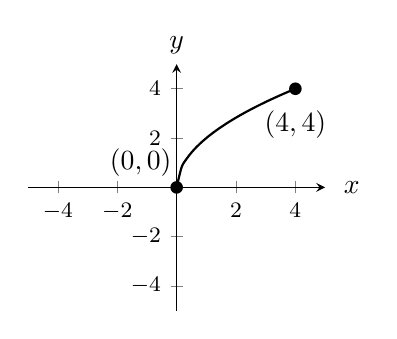
\begin{tikzpicture}
								\begin{axis}[
									scale=.55,
									every tick label/.append style={font=\footnotesize},
									axis x line = middle,
									axis y line = middle,
						    			every axis y label/.style={at={(ticklabel cs:1.15)}},
						    			%ytick = {-4, -2, -3, -1, 1, 2, 3, 4},
									y label style={at={(axis description cs:.5,1.15)},anchor=north},
						    			ylabel = {$y$},
						    			ymin = -5, ymax = 5,
					    				every axis x label/.style= {at ={(ticklabel cs:1)}},
					    				%xtick = {-4,-3,-2,-1,1,2,3,4},
					    				x label style={at={(axis description cs:1.15,.5)},anchor=east},
					    				xlabel = {$x$},
					    				xmin = -5, xmax = 5			
								]
									\addplot[thick, smooth,domain = 0:4] {2*sqrt(x)};
									\coordinate (p1) at (axis cs: 4,4);
									\coordinate (o) at (axis cs: 0,0);
								\end{axis}
								\fill (p1) circle (.08) node[yshift = -13pt] {$(4,4)$};
								\fill (o) circle (.08) node[yshift = 9pt, xshift=-13pt] {$(0,0)$};
							\end{tikzpicture} %vertical stretch
						\item 
							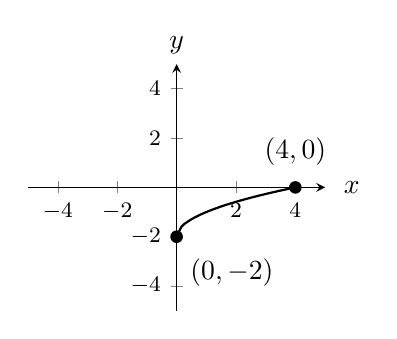
\begin{tikzpicture}
								\begin{axis}[
									scale=.55,
									every tick label/.append style={font=\footnotesize},
									axis x line = middle,
									axis y line = middle,
						    			every axis y label/.style={at={(ticklabel cs:1.15)}},
						    			%ytick = {-4, -2, -3, -1, 1, 2, 3, 4},
									y label style={at={(axis description cs:.5,1.15)},anchor=north},
						    			ylabel = {$y$},
						    			ymin = -5, ymax = 5,
					    				every axis x label/.style= {at ={(ticklabel cs:1)}},
					    				%xtick = {-4,-3,-2,-1,1,2,3,4},
					    				x label style={at={(axis description cs:1.15,.5)},anchor=east},
					    				xlabel = {$x$},
					    				xmin = -5, xmax = 5			
								]
									\addplot[thick, smooth,domain = 0:4] {sqrt(x)-2};
									\coordinate (p2) at (axis cs: 4,0);
									\coordinate (o2) at (axis cs: 0,-2);
								\end{axis}
								\fill (p2) circle (.08) node[yshift = 13pt] {$(4,0)$};
								\fill (o2) circle (.08) node[yshift = -13pt, xshift=20pt] {$(0,-2)$};
							\end{tikzpicture} %vertical shift
						\item 
							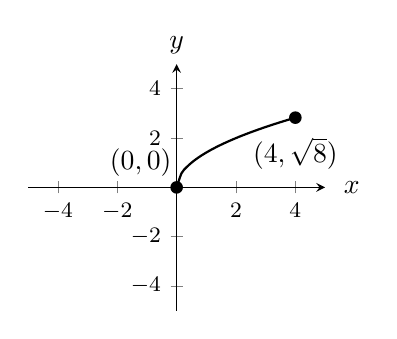
\begin{tikzpicture}
								\begin{axis}[
									scale=.55,
									every tick label/.append style={font=\footnotesize},
									axis x line = middle,
									axis y line = middle,
						    			every axis y label/.style={at={(ticklabel cs:1.15)}},
						    			%ytick = {-4, -2, -3, -1, 1, 2, 3, 4},
									y label style={at={(axis description cs:.5,1.15)},anchor=north},
						    			ylabel = {$y$},
						    			ymin = -5, ymax = 5,
					    				every axis x label/.style= {at ={(ticklabel cs:1)}},
					    				%xtick = {-4,-3,-2,-1,1,2,3,4},
					    				x label style={at={(axis description cs:1.15,.5)},anchor=east},
					    				xlabel = {$x$},
					    				xmin = -5, xmax = 5			
								]
									\addplot[thick, smooth,domain = 0:4] {sqrt(2*x)};
									\coordinate (p3) at (axis cs: 4,2.828);
									\coordinate (o) at (axis cs: 0,0);
								\end{axis}
								\fill (p3) circle (.08) node[yshift = -13pt] {$(4,\sqrt{8})$};
								\fill (o) circle (.08) node[yshift = 9pt, xshift=-13pt] {$(0,0)$};
							\end{tikzpicture} %horizontal shrink
						\item 
							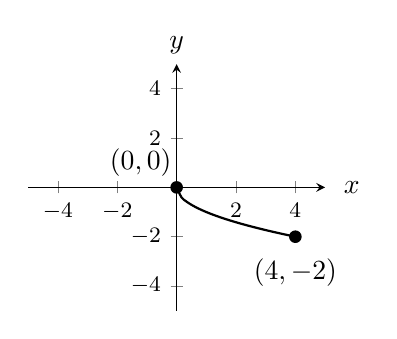
\begin{tikzpicture}
								\begin{axis}[
									scale=.55,
									every tick label/.append style={font=\footnotesize},
									axis x line = middle,
									axis y line = middle,
						    			every axis y label/.style={at={(ticklabel cs:1.15)}},
						    			%ytick = {-4, -2, -3, -1, 1, 2, 3, 4},
									y label style={at={(axis description cs:.5,1.15)},anchor=north},
						    			ylabel = {$y$},
						    			ymin = -5, ymax = 5,
					    				every axis x label/.style= {at ={(ticklabel cs:1)}},
					    				%xtick = {-4,-3,-2,-1,1,2,3,4},
					    				x label style={at={(axis description cs:1.15,.5)},anchor=east},
					    				xlabel = {$x$},
					    				xmin = -5, xmax = 5			
								]
									\addplot[thick, smooth,domain = 0:4] {-1*sqrt(x)};
									\coordinate (p4) at (axis cs: 4,-2);
									\coordinate (o) at (axis cs: 0,0);
								\end{axis}
								\fill (p4) circle (0.08) node[yshift = -13pt] {$(4,-2)$};
								\fill (o) circle (.08) node[yshift = 9pt, xshift=-13pt] {$(0,0)$};
							\end{tikzpicture} %reflection
								\columnbreak
						\item 
							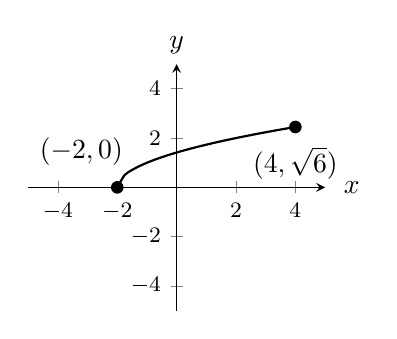
\begin{tikzpicture}
								\begin{axis}[
									scale=.55,
									every tick label/.append style={font=\footnotesize},
									axis x line = middle,
									axis y line = middle,
						    			every axis y label/.style={at={(ticklabel cs:1.15)}},
						    			%ytick = {-4, -2, -3, -1, 1, 2, 3, 4},
									y label style={at={(axis description cs:.5,1.15)},anchor=north},
						    			ylabel = {$y$},
						    			ymin = -5, ymax = 5,
					    				every axis x label/.style= {at ={(ticklabel cs:1)}},
					    				%xtick = {-4,-3,-2,-1,1,2,3,4},
					    				x label style={at={(axis description cs:1.15,.5)},anchor=east},
					    				xlabel = {$x$},
					    				xmin = -5, xmax = 5			
								]
									\addplot[thick, smooth,domain = -2:4] {sqrt(x+2)};
									\coordinate (p5) at (axis cs: 4, 2.449);
									\coordinate (o3) at (axis cs: -2,0);
								\end{axis}
								\fill (p5) circle (.08) node[yshift = -13pt] {$(4,\sqrt{6})$};
								\fill (o3) circle (.08) node[yshift = 13pt, xshift = -13pt] {$(-2,0)$};
							\end{tikzpicture} %horizontal shift
						\item 
							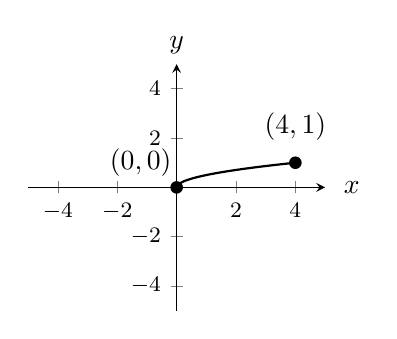
\begin{tikzpicture}
								\begin{axis}[
									scale=.55,
									every tick label/.append style={font=\footnotesize},
									axis x line = middle,
									axis y line = middle,
						    			every axis y label/.style={at={(ticklabel cs:1.15)}},
						    			%ytick = {-4, -2, -3, -1, 1, 2, 3, 4},
									y label style={at={(axis description cs:.5,1.15)},anchor=north},
						    			ylabel = {$y$},
						    			ymin = -5, ymax = 5,
					    				every axis x label/.style= {at ={(ticklabel cs:1)}},
					    				%xtick = {-4,-3,-2,-1,1,2,3,4},
					    				x label style={at={(axis description cs:1.15,.5)},anchor=east},
					    				xlabel = {$x$},
					    				xmin = -5, xmax = 5			
								]
									\addplot[thick, smooth,domain = 0:4] {(1/2)*sqrt(x)};
									\coordinate (p6) at (axis cs: 4,1);
									\coordinate (o) at (axis cs: 0,0);
								\end{axis}
								\fill (p6) circle (.08) node[yshift = 13pt] {$(4,1)$};
								\fill (o) circle (.08) node[yshift = 9pt, xshift=-13pt] {$(0,0)$};
							\end{tikzpicture} %vertical shrink
						\item 
							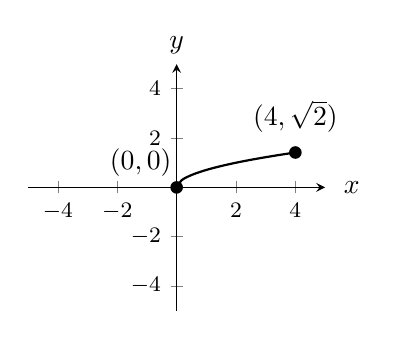
\begin{tikzpicture}
								\begin{axis}[
									scale=.55,
									every tick label/.append style={font=\footnotesize},
									axis x line = middle,
									axis y line = middle,
						    			every axis y label/.style={at={(ticklabel cs:1.15)}},
						    			%ytick = {-4, -2, -3, -1, 1, 2, 3, 4},
									y label style={at={(axis description cs:.5,1.15)},anchor=north},
						    			ylabel = {$y$},
						    			ymin = -5, ymax = 5,
					    				every axis x label/.style= {at ={(ticklabel cs:1)}},
					    				%xtick = {-4,-3,-2,-1,1,2,3,4},
					    				x label style={at={(axis description cs:1.15,.5)},anchor=east},
					    				xlabel = {$x$},
					    				xmin = -5, xmax = 5			
								]
									\addplot[thick, smooth,domain = 0:4] {sqrt(.5*x)};
									\coordinate (p7) at (axis cs: 4,1.414);
									\coordinate (o) at (axis cs: 0,0);
								\end{axis}
								\fill (p7) circle (.08) node[yshift = 13pt] {$(4,\sqrt{2})$};
								\fill (o) circle (.08) node[yshift = 9pt, xshift=-13pt] {$(0,0)$};
							\end{tikzpicture} %horizontal stretch
					\end{enumerate}
						\raggedcolumns
				\end{multicols*}
			\end{ex}
				\newpage
				
			\begin{ex}
				Sketch the graph of the function $f(x) = x^2 - 2x +3$ by applying transformations to the base graph of $f(x) = x^2$.
				\begin{center}
				\begin{tabu}{X[c]X[c]}
					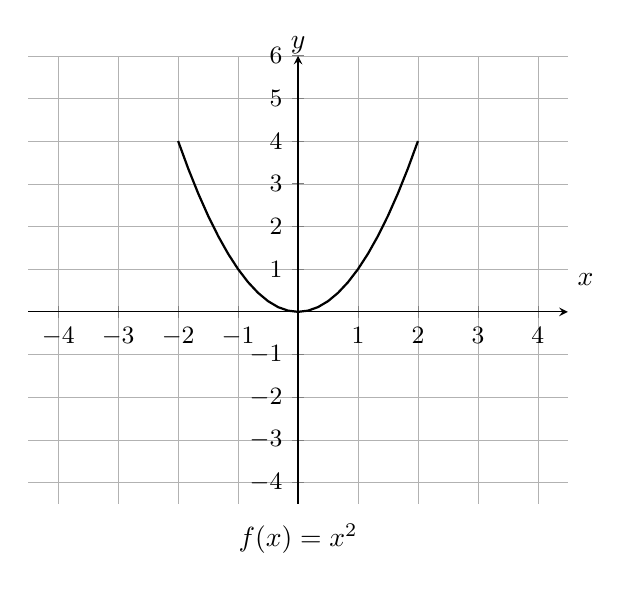
\begin{tikzpicture}
						\begin{axis}[
							grid style = {line width = .1pt, draw = gray!60},
							grid = both,
							every tick label/.append style={font=\small},
							axis x line = middle,
							axis y line = middle,
				    			every axis y label/.style={at={(ticklabel cs:1.15)}, yshift = -3pt},
								y label style={at={(axis description cs: 0.5, 1)},above},
							ytick = {-4,-3,-2,-1,1,2,3,4,5,6},
				    			ylabel = {$y$},
				    			ymin = -4.5, ymax = 6,
			    				every axis x label/.style= {at ={(ticklabel cs:1)}},
			    				xtick = {-4,-3,-2,-1,1,2,3,4},
				    				x label style={at={(axis description cs: 1, 0.5)},right},
			    				xlabel = {$x$},
			    				xmin = -4.5, xmax = 4.5,
						]
							\addplot[thick, domain = -2:2] {x^2};
							\coordinate (label) at (0,-5);
						\end{axis}						
						\draw (label) node[yshift = -5pt] {$f(x) = x^2$};
					\end{tikzpicture}
					&
					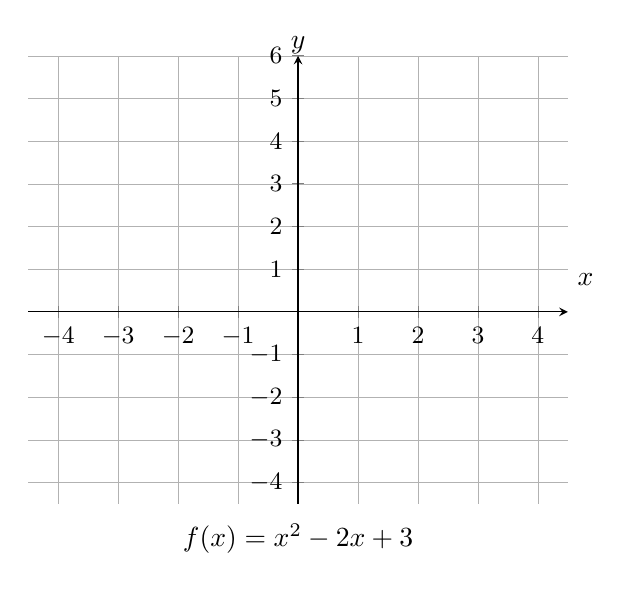
\begin{tikzpicture}
						\begin{axis}[
							grid style = {line width = .1pt, draw = gray!60},
							grid = both,
							every tick label/.append style={font=\small},
							axis x line = middle,
							axis y line = middle,
				    			every axis y label/.style={at={(ticklabel cs:1.15)}, yshift = -3pt},
								y label style={at={(axis description cs: 0.5, 1)},above},
							ytick = {-4,-3,-2,-1,1,2,3,4,5,6},
				    			ylabel = {$y$},
				    			ymin = -4.5, ymax = 6,
			    				every axis x label/.style= {at ={(ticklabel cs:1)}},
			    				xtick = {-4,-3,-2,-1,1,2,3,4},
				    				x label style={at={(axis description cs: 1, 0.5)},right},
			    				xlabel = {$x$},
			    				xmin = -4.5, xmax = 4.5
						]
							\coordinate (label) at (0,-5);
						\end{axis}
						\draw (label) node[yshift = -5pt] {$f(x) = x^2-2x+3$};
					\end{tikzpicture}
				\end{tabu}
				\end{center}
			\end{ex}
				\vs{.5}

		\begin{ex}
			Sketch the graphs of the given functions by using transformations to base graph:
			\begin{enumerate}[(a)]
				\item $f(x) = \dfrac{-2}{x+3}$
					\vs{1}
					\newpage
					
				\item $g(x) = 1-\cos 2x$
					\vs{1}
					
					
				\item $h(x) = |x^2-1|$
					\vs{2}
					
			\end{enumerate}				
		\end{ex}	
			
		\begin{rmk}[Function Composition]
			Given two function $f$ and $g$, the \textbf{composite function} $f\circ g$ is defined by \\
			\showto{ins}{
				\[(f\circ g)(x) = f(g(x))\]
			}
			\showto{st}{ \\ 
				\vspace{15pt}
			}
			The domain of $f\circ g$ is \showto{ins}{the set of all $x$ in the domain of $g$ such that $g(x)$ is in the domain of $f$.}\showto{st}{\blank{5}}.
		\end{rmk}
		
		\begin{ex}
			For each function below, (1) find the domain of the composite function, (2) completely decompose the function into smaller ones.
			\begin{enumerate}[(a)]
				\item $f(x) = \dfrac{1}{x+2}$
					\vs{1}
				
					\newpage
					
				\item  $q(x) = (2x+1)^5$		
					\vs{1}
						
				\item  $s(h) = \sin \left(5h^2 + \dfrac{1}{h}\right)$		
					\vs{1}
					
				\item  $y(r) = \dfrac{5.317}{(2r^5 + 1.7)^2}$		
					\vs{1}

				\item  $g(x) = \tan (x^2)$		
					\vs{1}
					
				
					
			\end{enumerate}
		\end{ex}
		
		\begin{ex}
			If $f(x) = \sqrt{x}$ and $g(x) = \sqrt{2-x}$, find 
				\begin{enumerate}[(a)]
					\item $f\circ g$
						\vs{1}
						
					\item $g\circ f$
						\vs{1}
						
					\item $f\circ f$
						\vs{1}
						
					\item $g\circ g$
						\vs{1}
				\end{enumerate}
		\end{ex}
			\newpage
			
		\begin{ex}
			Let $k(x) = \sec(x^2)\tan(x^2)$.  Find $f,g$ such that $k(x) = f(g(x))$.
		\end{ex}
			\vs{1}
			
		\begin{ex}
			Let $f(x) = \cos^2 (x^2 + 9)$.  Find functions $a,b,c$ such that $f(x) = (a\circ b\circ c)(x)$
		\end{ex}
			\vs{1}
		
		\begin{ex}
			Given $f(x) = x^2 + x -1$ and $g(x) = 2-x$, what is the equation of $y =(f\circ g)(x)$?
		\end{ex}
			\vs{1}
			
		\begin{ex}
			If $g(1) = 3$, then what point must be on the graph of $h(t) = -2g(t-1) + 6$?
		\end{ex}
			\vs{1}
			\newpage
		
	\subsection*{After Class}
	\addcontentsline{toc}{subsection}{After Class}		
		\begin{ex}
			For each function below, (i) identify the base graph, (ii) identify any transformation applied to the base graph, and (iii) sketch a rough graph of the function.
			\begin{enumerate}[(a)]
				\item $y = 2\cos 3x$
					\vs{1}

				\item $y = 3\sqrt{x+1}$
					\vs{1}
					
				\item $y = |\sqrt{x} - 1|$
					\vs{1}
					
			\end{enumerate}
		\end{ex}
			\newpage
			
		\begin{ex}
			Below is a table of input/output values for functions $f$ and $g$.
			\begin{center}
				\begin{tabular}{|c||c|c|c|c|c|c|}\hline
					$x$	&	1 	&	 2	& 	3	& 	4	& 	5	& 	6 \\ \hline
					$f(x)$&	3	& 	1	& 4		& 2		& 2 		& 5\\ \hline
					$g(x)$&	6	& 	3	& 2		& 1		& 2	& 3 \\ \hline
				\end{tabular}
			\end{center}
			Evaluate each expression below:
			\begin{enumerate}[(a)]
				\item $f(g(1))$
					\vs{.5}
					
				\item $g(f(1))$
					\vs{.5}
					
				\item $f(f(1))$
					\vs{.5}
					
				\item $g(g(1))$
					\vs{.5}
					
				\item $(g\circ f)(3)$
					\vs{.5}
					
				\item $(f\circ g)(6)$	
					\vs{.5}
			\end{enumerate}
		\end{ex}
			\newpage
			
		\begin{ex}
			If you invest $x$ dollars at at 6\% interest compounded annually, then the amount $A(x)$ of the investment after one year is $A(x) = 1.06x$.  
			\begin{enumerate}[(a)]
				\item Find $A\circ A\circ A\circ A$ and $A\circ A\circ A\circ A\circ A$.
					\vs{1}
					
				\item What do the compositions represent in real-world terms?
					\vs{1}
					
				\item Generalize your work in part (a); find a formula for the composition of $n$ copies of $A$.
					\vs{1}
					
			\end{enumerate}
		\end{ex}
		
		\begin{ex}
			If $g(x) = 2x + 1$ and $h(x) =4x^2 + 4x + 7$, find a function $f$ such that $f\circ g = h$.
		\end{ex}
			\vs{1}
			
	\clearpage
\end{document}